\documentclass{standalone}
\usepackage{tikz}
\usetikzlibrary{patterns, positioning}


\begin{document}
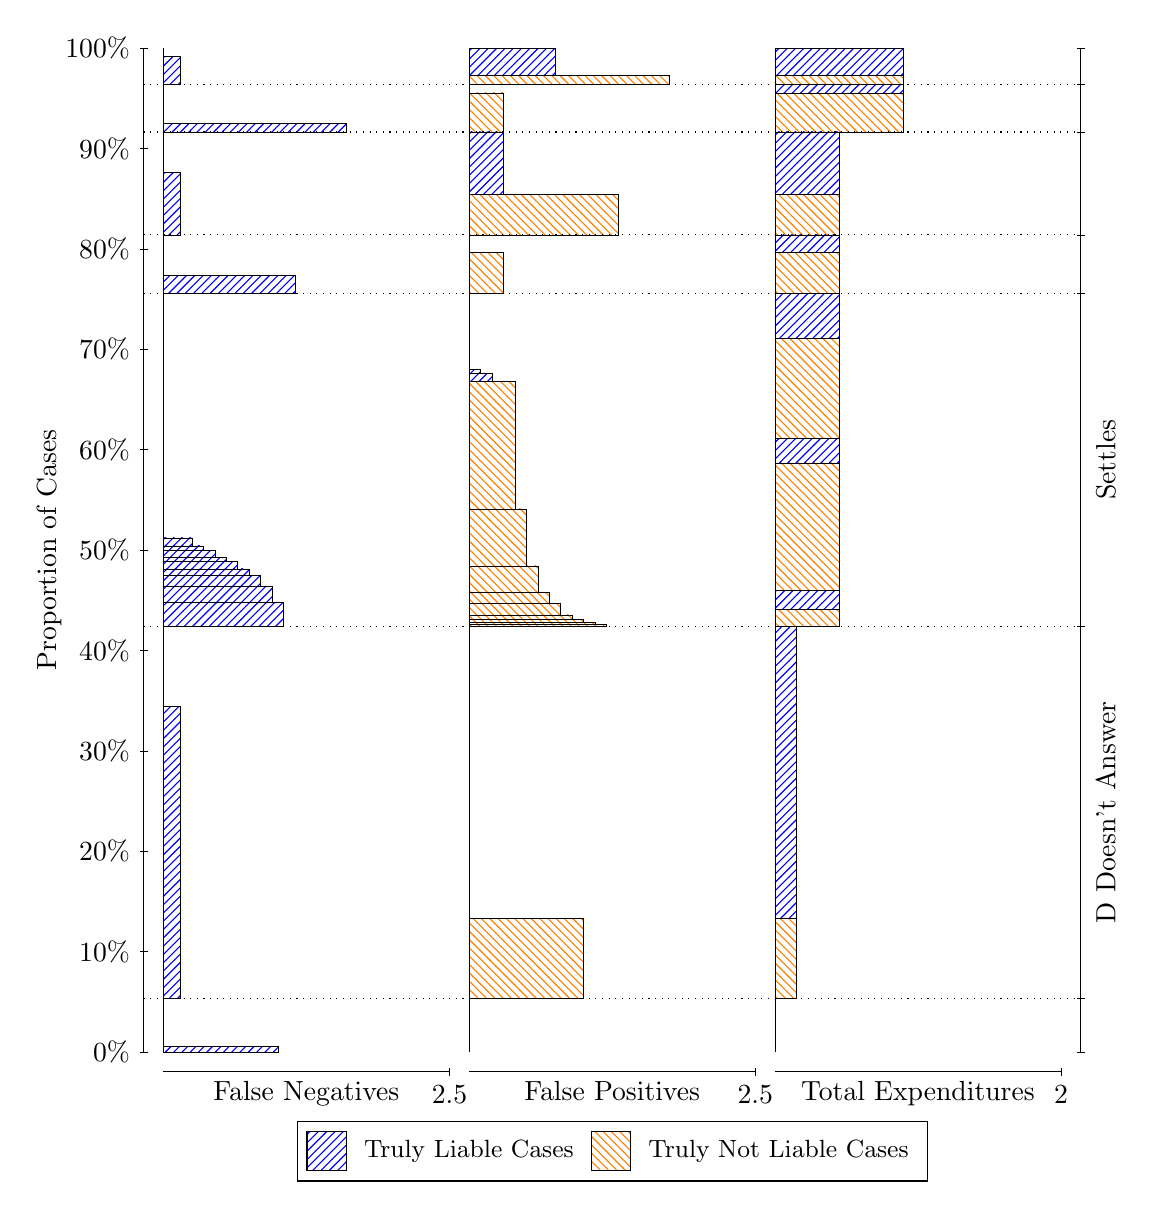
\begin{tikzpicture}
\draw[black, very thin] (1.5,1.75) -- (1.5,14.5);
\node[rotate=90, text=black, anchor=center] at (0.3, 8.125) {Proportion of Cases};
\draw[black, very thin] (1.45,1.75) -- (1.55,1.75);
\node[text=black, anchor=east] at (1.45, 1.75) {0\%};
\draw[black, very thin] (1.45,3.025) -- (1.55,3.025);
\node[text=black, anchor=east] at (1.45, 3.025) {10\%};
\draw[black, very thin] (1.45,4.3) -- (1.55,4.3);
\node[text=black, anchor=east] at (1.45, 4.3) {20\%};
\draw[black, very thin] (1.45,5.575) -- (1.55,5.575);
\node[text=black, anchor=east] at (1.45, 5.575) {30\%};
\draw[black, very thin] (1.45,6.85) -- (1.55,6.85);
\node[text=black, anchor=east] at (1.45, 6.85) {40\%};
\draw[black, very thin] (1.45,8.125) -- (1.55,8.125);
\node[text=black, anchor=east] at (1.45, 8.125) {50\%};
\draw[black, very thin] (1.45,9.4) -- (1.55,9.4);
\node[text=black, anchor=east] at (1.45, 9.4) {60\%};
\draw[black, very thin] (1.45,10.675) -- (1.55,10.675);
\node[text=black, anchor=east] at (1.45, 10.675) {70\%};
\draw[black, very thin] (1.45,11.95) -- (1.55,11.95);
\node[text=black, anchor=east] at (1.45, 11.95) {80\%};
\draw[black, very thin] (1.45,13.225) -- (1.55,13.225);
\node[text=black, anchor=east] at (1.45, 13.225) {90\%};
\draw[black, very thin] (1.45,14.5) -- (1.55,14.5);
\node[text=black, anchor=east] at (1.45, 14.5) {100\%};

\draw[black, very thin] (13.4,1.75) -- (13.4,14.5);
\draw[black, very thin] (13.35,1.75) -- (13.45,1.75);
\node[anchor=west] at (13.35, 1.75) {};
\draw[black, very thin] (13.35,2.4318) -- (13.45,2.4318);
\node[anchor=west] at (13.35, 2.4318) {};
\draw[black, very thin] (13.35,7.1557) -- (13.45,7.1557);
\node[anchor=west] at (13.35, 7.1557) {};
\draw[black, very thin] (13.35,11.386) -- (13.45,11.386);
\node[anchor=west] at (13.35, 11.386) {};
\draw[black, very thin] (13.35,12.128) -- (13.45,12.128);
\node[anchor=west] at (13.35, 12.128) {};
\draw[black, very thin] (13.35,13.434) -- (13.45,13.434);
\node[anchor=west] at (13.35, 13.434) {};
\draw[black, very thin] (13.35,14.042) -- (13.45,14.042);
\node[anchor=west] at (13.35, 14.042) {};
\draw[black, very thin] (13.35,14.5) -- (13.45,14.5);
\node[anchor=west] at (13.35, 14.5) {};

\draw[black, very thin, pattern color=blue, pattern=north east lines] (1.75,1.75) rectangle (3.2033,1.8217);
\draw[black, very thin, pattern color=orange, pattern=north west lines] (1.75,1.8217) rectangle (1.75,2.4318);
\draw[black, very thin, pattern color=blue, pattern=north east lines] (1.75,2.4318) rectangle (1.968,6.1368);
\draw[black, very thin, pattern color=orange, pattern=north west lines] (1.75,6.1368) rectangle (1.75,7.1557);
\draw[black, very thin, pattern color=blue, pattern=north east lines] (1.75,7.1557) rectangle (3.276,7.4617);
\draw[black, very thin, pattern color=blue, pattern=north east lines] (1.75,7.4617) rectangle (3.1307,7.6657);
\draw[black, very thin, pattern color=blue, pattern=north east lines] (1.75,7.6657) rectangle (2.9853,7.8059);
\draw[black, very thin, pattern color=blue, pattern=north east lines] (1.75,7.8059) rectangle (2.84,7.8859);
\draw[black, very thin, pattern color=blue, pattern=north east lines] (1.75,7.8859) rectangle (2.6947,7.9791);
\draw[black, very thin, pattern color=blue, pattern=north east lines] (1.75,7.9791) rectangle (2.5493,8.028);
\draw[black, very thin, pattern color=blue, pattern=north east lines] (1.75,8.028) rectangle (2.404,8.124);
\draw[black, very thin, pattern color=blue, pattern=north east lines] (1.75,8.124) rectangle (2.2587,8.1771);
\draw[black, very thin, pattern color=blue, pattern=north east lines] (1.75,8.1771) rectangle (2.1133,8.2778);
\draw[black, very thin, pattern color=orange, pattern=north west lines] (1.75,8.2778) rectangle (1.75,11.386);
\draw[black, very thin, pattern color=blue, pattern=north east lines] (1.75,11.386) rectangle (3.4213,11.611);
\draw[black, very thin, pattern color=orange, pattern=north west lines] (1.75,11.611) rectangle (1.75,12.128);
\draw[black, very thin, pattern color=blue, pattern=north east lines] (1.75,12.128) rectangle (1.968,12.92);
\draw[black, very thin, pattern color=orange, pattern=north west lines] (1.75,12.92) rectangle (1.75,13.434);
\draw[black, very thin, pattern color=blue, pattern=north east lines] (1.75,13.434) rectangle (4.0753,13.546);
\draw[black, very thin, pattern color=orange, pattern=north west lines] (1.75,13.546) rectangle (1.75,14.042);
\draw[black, very thin, pattern color=blue, pattern=north east lines] (1.75,14.042) rectangle (1.968,14.389);
\draw[black, very thin, pattern color=orange, pattern=north west lines] (1.75,14.389) rectangle (1.75,14.5);
\draw[black, very thin, pattern color=orange, pattern=north west lines] (5.6333,1.75) rectangle (5.6333,2.3601);
\draw[black, very thin, pattern color=blue, pattern=north east lines] (5.6333,2.3601) rectangle (5.6333,2.4318);
\draw[black, very thin, pattern color=orange, pattern=north west lines] (5.6333,2.4318) rectangle (7.0867,3.4508);
\draw[black, very thin, pattern color=blue, pattern=north east lines] (5.6333,3.4508) rectangle (5.6333,7.1557);
\draw[black, very thin, pattern color=orange, pattern=north west lines] (5.6333,7.1557) rectangle (7.3773,7.1791);
\draw[black, very thin, pattern color=orange, pattern=north west lines] (5.6333,7.1791) rectangle (7.232,7.2029);
\draw[black, very thin, pattern color=orange, pattern=north west lines] (5.6333,7.2029) rectangle (7.0867,7.2481);
\draw[black, very thin, pattern color=orange, pattern=north west lines] (5.6333,7.2481) rectangle (6.9413,7.3004);
\draw[black, very thin, pattern color=orange, pattern=north west lines] (5.6333,7.3004) rectangle (6.796,7.4497);
\draw[black, very thin, pattern color=orange, pattern=north west lines] (5.6333,7.4497) rectangle (6.6507,7.5891);
\draw[black, very thin, pattern color=orange, pattern=north west lines] (5.6333,7.5891) rectangle (6.5053,7.9244);
\draw[black, very thin, pattern color=orange, pattern=north west lines] (5.6333,7.9244) rectangle (6.36,8.6475);
\draw[black, very thin, pattern color=orange, pattern=north west lines] (5.6333,8.6475) rectangle (6.2147,10.264);
\draw[black, very thin, pattern color=blue, pattern=north east lines] (5.6333,10.264) rectangle (5.924,10.365);
\draw[black, very thin, pattern color=blue, pattern=north east lines] (5.6333,10.365) rectangle (5.7787,10.418);
\draw[black, very thin, pattern color=blue, pattern=north east lines] (5.6333,10.418) rectangle (5.6333,11.386);
\draw[black, very thin, pattern color=orange, pattern=north west lines] (5.6333,11.386) rectangle (6.0693,11.902);
\draw[black, very thin, pattern color=blue, pattern=north east lines] (5.6333,11.902) rectangle (5.6333,12.128);
\draw[black, very thin, pattern color=orange, pattern=north west lines] (5.6333,12.128) rectangle (7.5227,12.642);
\draw[black, very thin, pattern color=blue, pattern=north east lines] (5.6333,12.642) rectangle (6.0693,13.434);
\draw[black, very thin, pattern color=orange, pattern=north west lines] (5.6333,13.434) rectangle (6.0693,13.931);
\draw[black, very thin, pattern color=blue, pattern=north east lines] (5.6333,13.931) rectangle (5.6333,14.042);
\draw[black, very thin, pattern color=orange, pattern=north west lines] (5.6333,14.042) rectangle (8.1767,14.153);
\draw[black, very thin, pattern color=blue, pattern=north east lines] (5.6333,14.153) rectangle (6.7233,14.5);
\draw[black, very thin, pattern color=orange, pattern=north west lines] (9.5167,1.75) rectangle (9.5167,2.3601);
\draw[black, very thin, pattern color=blue, pattern=north east lines] (9.5167,2.3601) rectangle (9.5167,2.4318);
\draw[black, very thin, pattern color=orange, pattern=north west lines] (9.5167,2.4318) rectangle (9.7892,3.4508);
\draw[black, very thin, pattern color=blue, pattern=north east lines] (9.5167,3.4508) rectangle (9.7892,7.1557);
\draw[black, very thin, pattern color=orange, pattern=north west lines] (9.5167,7.1557) rectangle (10.334,7.374);
\draw[black, very thin, pattern color=blue, pattern=north east lines] (9.5167,7.374) rectangle (10.334,7.6163);
\draw[black, very thin, pattern color=orange, pattern=north west lines] (9.5167,7.6163) rectangle (10.334,9.2326);
\draw[black, very thin, pattern color=blue, pattern=north east lines] (9.5167,9.2326) rectangle (10.334,9.5386);
\draw[black, very thin, pattern color=orange, pattern=north west lines] (9.5167,9.5386) rectangle (10.334,10.812);
\draw[black, very thin, pattern color=blue, pattern=north east lines] (9.5167,10.812) rectangle (10.334,11.386);
\draw[black, very thin, pattern color=orange, pattern=north west lines] (9.5167,11.386) rectangle (10.334,11.902);
\draw[black, very thin, pattern color=blue, pattern=north east lines] (9.5167,11.902) rectangle (10.334,12.128);
\draw[black, very thin, pattern color=orange, pattern=north west lines] (9.5167,12.128) rectangle (10.334,12.642);
\draw[black, very thin, pattern color=blue, pattern=north east lines] (9.5167,12.642) rectangle (10.334,13.434);
\draw[black, very thin, pattern color=orange, pattern=north west lines] (9.5167,13.434) rectangle (11.152,13.931);
\draw[black, very thin, pattern color=blue, pattern=north east lines] (9.5167,13.931) rectangle (11.152,14.042);
\draw[black, very thin, pattern color=orange, pattern=north west lines] (9.5167,14.042) rectangle (11.152,14.153);
\draw[black, very thin, pattern color=blue, pattern=north east lines] (9.5167,14.153) rectangle (11.152,14.5);
\draw[black, dotted] (1.5,2.4318) -- (13.4,2.4318);
\draw[black, dotted] (1.5,7.1557) -- (13.4,7.1557);
\draw[black, dotted] (1.5,11.386) -- (13.4,11.386);
\draw[black, dotted] (1.5,12.128) -- (13.4,12.128);
\draw[black, dotted] (1.5,13.434) -- (13.4,13.434);
\draw[black, dotted] (1.5,14.042) -- (13.4,14.042);
\draw[black, very thin] (1.75,1.5) -- (5.3833,1.5);
\node[text=black, anchor=north] at (3.5667, 1.5) {False Negatives};
\draw[black, very thin] (5.3833,1.45) -- (5.3833,1.55);
\node[text=black, anchor=north] at (5.3833, 1.45) {2.5};

\draw[black, very thin] (5.6333,1.5) -- (9.2667,1.5);
\node[text=black, anchor=north] at (7.45, 1.5) {False Positives};
\draw[black, very thin] (9.2667,1.45) -- (9.2667,1.55);
\node[text=black, anchor=north] at (9.2667, 1.45) {2.5};

\draw[black, very thin] (9.5167,1.5) -- (13.15,1.5);
\node[text=black, anchor=north] at (11.333, 1.5) {Total Expenditures};
\draw[black, very thin] (13.15,1.45) -- (13.15,1.55);
\node[text=black, anchor=north] at (13.15, 1.45) {2};


\node[text=black, centered, rotate=90] at (13.72, 4.7938) {D Doesn't Answer};
\node[text=black, centered, rotate=90] at (13.72, 9.2708) {Settles};





\draw (7.449999999999999,1.5) node[draw=none] (baseCoordinate) {};
\begin{scope}[align=center]
        \matrix[scale=0.5, draw=black, below=0.5cm of baseCoordinate, nodes={draw}, column sep=0.1cm]{
            \node[rectangle, draw, minimum width=0.5cm, minimum height=0.5cm, pattern color=blue, pattern=north east lines] {}; &
            \node[draw=none, font=\small, text=black] (B) {Truly Liable Cases}; &
            \node[rectangle, draw, minimum width=0.5cm, minimum height=0.5cm, pattern color=orange, pattern=north west lines] {}; &
            \node[draw=none, font=\small, text=black] (B) {Truly Not Liable Cases}; \\
            };
\end{scope}

\end{tikzpicture}
\end{document}